\documentclass{article}
\usepackage{geometry}
\usepackage{amsmath}
\usepackage{amssymb}
\usepackage{array}
\usepackage{tabularx}
\usepackage{setspace}
\usepackage{graphicx}
\usepackage{tikz}
\usepackage{fancyhdr}

\geometry{a4paper, margin=1in}
\setlength{\headheight}{33pt}
\addtolength{\topmargin}{-21pt}

% --- Watermark setup ---
\usepackage{eso-pic}
\newcommand\BackgroundPicture{%
\put(\LenToUnit{0.5\paperwidth},\LenToUnit{0.5\paperheight}){%
\makebox(0,0)[c]{%
\tikz[opacity=0.08]\node{\includegraphics[width=1\paperwidth]{../oatutors_logo.png}};%
}%
}}
\AddToShipoutPicture{\BackgroundPicture}
% --- End Watermark setup ---

% --- Header setup for logo ---
\pagestyle{fancy}
\fancyhf{}
\fancyhead[L]{\includegraphics[height=1.0cm]{../oatutors_logo.png}}
\fancyhead[C]{\textbf{11+ Mathematics}}
\fancyhead[R]{\rightmark}
\fancyfoot[C]{\thepage}
\renewcommand{\headrulewidth}{0.4pt}
\renewcommand{\footrulewidth}{0.4pt}
% --- End Header setup ---

\begin{document}
\onehalfspacing

\begin{center}
\textbf{\Large 11+ Maths: Number Properties \& Special Numbers}
\vspace{0.2cm}
\end{center}

\hrule
\vspace{0.1cm}

\textbf{Topic:} Even, Odd, Prime, Composite, Triangular, Square, Cube Numbers \\
\textbf{Target Age:} 10-11 years (Preparing for 11+ Exams) \\
\textbf{Time:} 60 Minutes \\
\textbf{Resources:} Number grids, dot patterns, factor trees \\
\textbf{Website:} \texttt{https://oatutors.co.uk/}

\vspace{0.2cm}
\hrule
\vspace{0.3cm}

This lesson explores the fascinating world of number properties and special number families - crucial knowledge for 11+ pattern questions and number theory problems.

\section{Learning Objectives}
By the end of this lesson, students will be able to:
\begin{itemize}
    \item Identify even and odd numbers and understand their properties
    \item Recognize prime and composite numbers up to 100
    \item Calculate and identify square numbers and cube numbers
    \item Understand triangular numbers and their patterns
    \item Apply number properties to solve 11+ problems
    \item Use systematic methods to test number properties
\end{itemize}

\section{Starter Activity (10 Minutes)}

\begin{tabularx}{\textwidth}{|>{\raggedright\arraybackslash}p{1cm}|>{\raggedright\arraybackslash}p{3cm}|>{\raggedright\arraybackslash}X|}
\hline
\textbf{Time} & \textbf{Activity} & \textbf{Description} \\
\hline
5 mins & Number Properties Bingo & Call out properties: "A prime number less than 10", "A square number between 20 and 30". Students mark numbers on their grids. \\
\hline
5 mins & Pattern Spotting & Show sequence: 1, 4, 9, 16, 25... Students identify the pattern and predict next terms. \\
\hline
\end{tabularx}

\section{Main Teaching (25 Minutes)}

\subsection{Even and Odd Numbers (5 minutes)}

\textbf{Definitions:}
\begin{itemize}
    \item \textbf{Even numbers:} Divisible by 2 (end in 0, 2, 4, 6, 8)
    \item \textbf{Odd numbers:} Not divisible by 2 (end in 1, 3, 5, 7, 9)
\end{itemize}

\textbf{Key Properties for 11+:}
\begin{itemize}
    \item Even + Even = Even
    \item Odd + Odd = Even  
    \item Even + Odd = Odd
    \item Even × Any number = Even
    \item Odd × Odd = Odd
\end{itemize}

\subsection{Prime and Composite Numbers (8 minutes)}

\textbf{Prime Numbers:} Numbers with exactly 2 factors (1 and itself)
\begin{center}
First 10 primes: 2, 3, 5, 7, 11, 13, 17, 19, 23, 29
\end{center}

\textbf{Key Points:}
\begin{itemize}
    \item 1 is neither prime nor composite
    \item 2 is the only even prime number
    \item All other primes are odd
\end{itemize}

\textbf{Composite Numbers:} Numbers with more than 2 factors
\begin{center}
Examples: 4, 6, 8, 9, 10, 12, 14, 15, 16, 18, 20...
\end{center}

\textbf{Testing for Primes - 11+ Method:}
To test if a number n is prime, check if it's divisible by any prime up to $\sqrt{n}$.

\subsection{Square Numbers (4 minutes)}

\textbf{Definition:} A number multiplied by itself
\begin{center}
$1^2 = 1$, $2^2 = 4$, $3^2 = 9$, $4^2 = 16$, $5^2 = 25$, $6^2 = 36$, $7^2 = 49$, $8^2 = 64$, $9^2 = 81$, $10^2 = 100$
\end{center}

\textbf{Visual Pattern:}
\begin{center}
\begin{tikzpicture}[scale=0.4]
% 1^2
\fill (0,0) rectangle (0.8,0.8);
\node at (0.4,-0.3) {$1^2$};

% 2^2  
\fill (2,0) rectangle (2.8,0.8);
\fill (2.8,0) rectangle (3.6,0.8);
\fill (2,0.8) rectangle (2.8,1.6);
\fill (2.8,0.8) rectangle (3.6,1.6);
\node at (2.8,-0.3) {$2^2$};

% 3^2
\draw (5,0) grid (8,3);
\node at (6.5,-0.3) {$3^2$};
\end{tikzpicture}
\end{center}

\subsection{Cube Numbers (4 minutes)}

\textbf{Definition:} A number multiplied by itself three times
\begin{center}
$1^3 = 1$, $2^3 = 8$, $3^3 = 27$, $4^3 = 64$, $5^3 = 125$, $6^3 = 216$
\end{center}

\textbf{Memory Aid:} Think of building cubes with unit blocks.

\subsection{Triangular Numbers (4 minutes)}

\textbf{Definition:} Numbers that can form triangular patterns
\begin{center}
T$_1$ = 1, T$_2$ = 3, T$_3$ = 6, T$_4$ = 10, T$_5$ = 15, T$_6$ = 21
\end{center}

\textbf{Visual Pattern:}
\begin{center}
\begin{tikzpicture}[scale=0.3]
% T1
\fill (0,0) circle (0.1);
\node at (0,-0.5) {T$_1$=1};

% T2
\fill (2,0) circle (0.1);
\fill (1.5,0.5) circle (0.1);
\fill (2.5,0.5) circle (0.1);
\node at (2,-0.5) {T$_2$=3};

% T3
\fill (4,0) circle (0.1);
\fill (4.5,0) circle (0.1);
\fill (5,0) circle (0.1);
\fill (4.25,0.5) circle (0.1);
\fill (4.75,0.5) circle (0.1);
\fill (4.5,1) circle (0.1);
\node at (4.5,-0.5) {T$_3$=6};
\end{tikzpicture}
\end{center}

\textbf{Formula:} T$_n$ = $\frac{n(n+1)}{2}$

\section{Guided Practice (15 Minutes)}

\subsection*{Worksheet: Number Properties Investigation}

\textbf{Section A: Basic Properties (5 minutes)}
\begin{enumerate}
    \item Circle the prime numbers: 11, 15, 17, 21, 23, 27, 29
    \item Which of these are square numbers? 36, 48, 49, 63, 64, 81
    \item List the first 6 triangular numbers
    \item What type of number is 27? (Give all possible descriptions)
\end{enumerate}

\textbf{Section B: Problem Solving (7 minutes)}
\begin{enumerate}
    \setcounter{enumi}{4}
    \item Is 91 prime or composite? Show your working.
    \item Find a number that is both square and triangular.
    \item The sum of two consecutive odd numbers is 48. What are the numbers?
    \item Which prime number is one less than a square number?
\end{enumerate}

\textbf{Section C: Pattern Extension (3 minutes)}
\begin{enumerate}
    \setcounter{enumi}{8}
    \item Continue the sequence: 1, 8, 27, 64, \_\_\_, \_\_\_
    \item What's the 10th triangular number?
\end{enumerate}

\section{Independent Work (8 Minutes)}

\textbf{11+ Challenge Problems:}
\begin{enumerate}
    \item A number is both a square number and a cube number. What is the smallest such positive number greater than 1?
    \item How many prime numbers are there between 50 and 100?
    \item Find three consecutive numbers where the middle one is a square number.
    \item A triangular number plus 1 gives a square number. Find the first three examples.
\end{enumerate}

\section{Plenary and Assessment (2 Minutes)}

\begin{tabularx}{\textwidth}{|>{\raggedright\arraybackslash}p{1cm}|>{\raggedright\arraybackslash}p{3cm}|>{\raggedright\arraybackslash}X|}
\hline
\textbf{Time} & \textbf{Activity} & \textbf{Description} \\
\hline
2 mins & Properties Quiz & Quick-fire: "Name a prime between 40 and 50", "What's $8^2$?", "Is 51 prime?" Check understanding. \\
\hline
\end{tabularx}

\section{Homework Assignment}

\textbf{Special Numbers Investigation:}
\begin{enumerate}
    \item Create factor trees for numbers 24, 36, 48, 60
    \item Find all prime numbers up to 50 using Sieve of Eratosthenes
    \item Calculate the first 10 square numbers and first 8 cube numbers
    \item Research: Find 3 interesting facts about the number 1729
    \item Extension: Investigate perfect numbers (numbers equal to sum of proper factors)
\end{enumerate}

\section{Extension Activities}

For more able students:
\begin{itemize}
    \item Explore Fermat primes and Mersenne primes
    \item Investigate pentagonal and hexagonal numbers
    \item Research twin primes and goldbach's conjecture
    \item Create visual proofs for square number patterns
\end{itemize}

\newpage

\section*{Answer Key - For Teachers}

\subsection*{Guided Practice Answers}

\textbf{Section A: Basic Properties}
\begin{enumerate}
    \item Prime numbers: 11, 17, 23, 29
    \item Square numbers: 36 (6²), 49 (7²), 64 (8²), 81 (9²)
    \item Triangular numbers: 1, 3, 6, 10, 15, 21
    \item 27: Odd, composite, cube number (3³)
\end{enumerate}

\textbf{Section B: Problem Solving}
\begin{enumerate}
    \setcounter{enumi}{4}
    \item 91 = 7 × 13, so composite
    \item 36 (6² and T₈)
    \item 23 and 25 (consecutive odd numbers)
    \item 3 (which is one less than 4 = 2²)
\end{enumerate}

\textbf{Section C: Pattern Extension}
\begin{enumerate}
    \setcounter{enumi}{8}
    \item 125, 216 (cube numbers: 5³, 6³)
    \item T₁₀ = 55
\end{enumerate}

\subsection*{Independent Work Answers}
\begin{enumerate}
    \item 64 (8² = 4³ = 64)
    \item 10 prime numbers (53, 59, 61, 67, 71, 73, 79, 83, 89, 97)
    \item 8, 9, 10 (where 9 = 3²)
    \item T₃ + 1 = 7 (not square), T₈ + 1 = 37 (not square), T₄₉ + 1 = 50² (1225 + 1 = 1226... need to check systematically)
\end{enumerate}

\subsection*{Teaching Notes}
\begin{itemize}
    \item Use visual aids extensively - dot patterns work well
    \item Common misconception: Students think 1 is prime
    \item Emphasize systematic checking methods for 11+ exams
    \item Connect to real-world applications (cryptography, tiling patterns)
    \item Use games and competitions to maintain engagement
\item Practice recognition speed - 11+ exams require quick identification
\end{itemize}

\end{document}